%%=============================================================================
%% Methodologie
%%=============================================================================

\chapter{\IfLanguageName{dutch}{Methodologie}{Methodology}}%
\label{ch:methodologie}

In deze bachelorproef wordt er een onderzoek op kwalitatieve en kwantitatieve wijze uitgevoerd. Op deze manier trachten we de volgende onderzoeksvraag te beantwoorden: "Kan GraphQL of een soortgelijke oplossing geïmplementeerd worden in een zelfontwikkelde accelerator?".

Dit gebeurt als start door het uitvoeren van een literatuurstudie die terug te vinden is in hoofdstuk 2 onder Stand van zaken. De implementatie en bjihorende uitwerkingen zijn zowel in een thuisnetwerk evenals in een bedrijfsnetwerk uitgevoerd. Hiervoor was van Delaware uit hardware en een werkomgeving voorzien met de benodigde licenties om dit te realiseren. Dit werd ondersteund door het Delaware Microsoft Integration team.

\section{\IfLanguageName{dutch}{Testomgeving}{Testomgeving}}%
\label{sec:Testomgeving}

De literatuurstudie omschrijft wat de Data-Accelerator exact is en hoe deze in hun workflow gebruikt wordt. Hierbij werden de benodigde begrippen uitgelegd om dit een vorm te geven. Dit wordt ondersteund door wetenschappelijke artikels en handleidingen opgesteld door softwareontwikkelaars. Deze werden geraadpleegd via Google Scholar en de bibliotheek van HoGent en UGent. Binnen Delaware was de code van de Data-Accelerator software en een korte demo voorzien om snel wegwijs te geraken met diens toepassingen.

Echter om deze Data-Accelerator te gebruiken moet er omgeving opgezet worden in Microsoft Azure. Aan de hand van die korte demo werd er een kant en klare omgeving opgesteld, gebruikmakend van Azure Pipelines om via YAML code deze tot een correcte werking te stellen.

Om deze pipeline uit te voeren moesten er ook BICEP bestanden aangemaakt worden, deze zijn code-gebaseerde bestanden toegepspitst op een deel van de omgeving die benodigd is zoals een databank. Deze zijn getest qua functionaliteit door Dhr. Dedeken zelf om legitimiteit toe te kennen aan de opgezette omgeving. Zodat dit onderzoek binnen de bachelorproef een beter beeld oplevert.

\section{\IfLanguageName{dutch}{verloop}{verloop}}%
\label{sec:Verloop}

Na het uitwerken van de literatuurstudie is dit onderzoek gecontinueerd met het configureren en opzetten van de benodigde services. Dit bestaat uit het documenteren van alle klassen en functies binnen de Data-Accelerator, aangezien dit nog niet aanwezig was. Op die manier kon de interne werking van de Data-Accelerator bestudeerd worden en was er controle van Dhr. Dedeken uit om mogelijke interpretatie fouten te corrigeren. Dit wordt dan ook de documenteerfase genoemd binnen het onderzoek. De documentatie werd ook geschreven aan de hand van XML bijschriften bij elke functie en klasse binnen de 53 klassen die samen de Data-Accelerator vormen.

Het volgende deel van de uitwerking was om de gehele omgeving manueel op te zetten binnen Azure met als doel een eerste blik op de werking van de Data-Accelerator te krijgen en zijn functies te testen. Hierbij werden verschillende resources binneen Azure opgezet en voorzien van benodigde data en instellingen om een werkend geheel te vormen. Dit vormt dan ook de basis om de BICEP bestanden op te stellen.

Vervolgens werden BICEP templates opgesteld die via enkele globaal gedefineerde parameters een omgeving konden opzetten. Hiervoor werden van de manuele opgezette omgeving in Azure ARM templates gegenereerd. Deze zijn dan manueel omgevormd tot BICEP templates vanwege de herbruikbaarheid in meerdere omgevingen. De keuze voor BICEP kwam er doordat als men zich bij ARM templates houdt en er loopt iets mis bij het opzetten van de omgeving, deze alle voorgaande data verwijderd. Dit is catastrofaal bij een project met klanten die hier volledig rond opgezet zijn.

Het volgende deel was het opstellen van een pipeline in YAML die via Azure Pipelines uitgevoerd kon worden. Hierin werden parameters meegegeven die personaliseerbaar gemaakt zijn om zo bij verschillende omgevingen correcte naamgeving en specificaties te hebben. In deze pipeline worden dan ook de BICEP templates gecontroleerd op syntaxfouten en indien alles correct bevonden is, uitgevoerd. Hierbij wordt er ook gebruik gemaakt van de Azure Command Line Interface om delen te voorzien. Er wordt ook een PowerShell script uitgevoerd om de benodigde databank in deze opstelling te voorzien van data. In een productieomgeving zal dit beschikbaar gesteld worden door de werkgever maar voor dit onderzoek is er één gecreëerd.

Als voorlaatste deel van dit onderzoek werd er dan gekeken hoe men GraphQL of soortgelijke functionaliteit kon toevoegen om deze software uit te breiden. Hiervoor is er ook gekeken naar mogelijke services die al reeds door Azure voorzien zijn. Stel dat dit mogelijk is, kan de reeds bestaande omgeving snel uitgebreid en ook geautomatiseerd worden via de vooropgestelde pipeline om een vlotte opzet bij projecten te garanderen.

Het onderzoek werd afgesloten met een test van de omgeving en of deze samen kon werken met de Data-Accelerator om zo een extra tool bij het Zwitsers zakmes toe te voegen. Dit wordt vervolgens verwerkt tot een gepaste conclusie binnen deze bachelorproef.

\subsection{\IfLanguageName{dutch}{Documentatie}{Documentatie}}%
\label{sec:Documentatie}

Voordat er een omgeving opgesteld wordt moet de code eerst beschreven worden van de Data-Accelerator. Dit gebeurd aan de hand van XML beschrijvingen bij elke functie en klasse die de accelerator omvat. Deze bestond uit 53 klassen die elk meerdere functies bevat. Deze zijn terug te vinden in bijlage B.4 Documentatie. Het eerste deel van deze klassen zijn gegroepeerd volgens hun functie namelijk: Activiteiten, Entrypoints en Orchestratie. Het tweede deel werd dan gegroepeerd op basis van hun ondersteuning. Deze zijn: Communitcatie, Conversie, Helpers, Interfaces, IOC, SQL, Storage en XSLT. De XML beschrijvingen bij elke functie of klasse bestonden uit hun samenvatting, gebruikte parameters, wat deze juist inhouden en wat er mogelijks kon geresulteerd worden bij een functie.

\subsection{\IfLanguageName{dutch}{BICEP}{BICEP}}%
\label{sec:BICEP}

Om de Data-Accelerator te kunnen gebruiken werden in Microsoft Azure binnen een Resource Group de volgende omgevingen aangemaakt die ook zichtbaar zijn in bijlage B.5 Azure:

Een SQL database om de data die gebruikt wordt door de Data-Accelerator bij te houden.

Application Insights om de performantie van de applicatie te monitoren.

Een Managed Identity om de gebruiker van de Resource Group de gepaste rechten toe te wijzen in verband met aanpassingen doorvoeren en de pipeline te kunnen uitvoeren.

Een SQL server om toegang tot de databank te beperken tot geselecteerde IP-adressen.

Een Virtual network om een bedrijfsnetwerk te simuleren, want dit wordt bij klanten voorzien en toegepast.

Het Storage Account waarin alle containers die benodigd zijn aangemaakt worden. Hierin zijn de scripts, queries en XSLT bestanden geplaatst zodat in het geval van een lokaal verlies van de bestanden deze ergens veilig te vinden zijn. Dit bevat alle Azure Storage data objects zoals blobs, schijven, tables en gedeelde bestanden.

Er is ook een Private DNS zone ogezet om bij het gebruik van een Virtual network er ook een DNS zone aan gekoppeld kan worden.

Als laatste is er een Keyvault toegevoegd. Deze bevat aanmeldingsgegevens en andere waarden die versleuteld zijn zodat die dan in de pipeline opgehaald en gebruikt kunnen worden op een veilige manier.

Na het opstellen van deze omgeving manueel, zijn de hierboven benoemde delen omgezet naar ARM templates. Deze zijn op hun beurt omgevormd tot BICEP templates vanwege de hiervoor benoemde problemen die zich kunnen voordoen bij ARM. De templates zijn zodanig opgesteld dat ze automatisch de juiste naamgeving bevatten en samen kunnen werken. Deze zijn zichtbaar in bijlage B.6 BICEP.

\subsection{\IfLanguageName{dutch}{Pipeline}{Pipeline}}%
\label{sec:Pipeline}

De BICEP bestanden die in voorgaande stage van de uitwerking aangemaakt zijn. Moeten nu via een pipeline geïntegrerd worden in Azure om zo de gehele omgeving op te zetten. Deze pipeline is te vinden in bijlage B.7 YAML. Deze is opgesteld met parameters die geïmporteerd worden uit een ander bestand zodat men deze kan personaliseren per omgeving waarin men de Data-Accelerator wenst te gebruiken. Hierdoor kan men aan de pipeline zelf niks veranderen maar wel de benamingen en specificaties doorgeven aan de BICEP templates, Azure Command Line Interface en het PowerShell script.

Eerst en vooral ziet men bovenaan het script enkele parameters staat die men dan kan selecteren om de omgeving naar wens op te zetten. Deze parameters omvatten de opties om een Virtual network aan te maken, de databank op te vullen met test data, de XSLT mappings en queries die men wilt uitvoeren met de Data-Accelerator op te slaan in het Storage Account en de Resource Group waarin men wilt te werk gaan. Dit kan teruggevonden worden in Figuur~\ref{fig:Opties}.

\begin{figure}
    \centering
    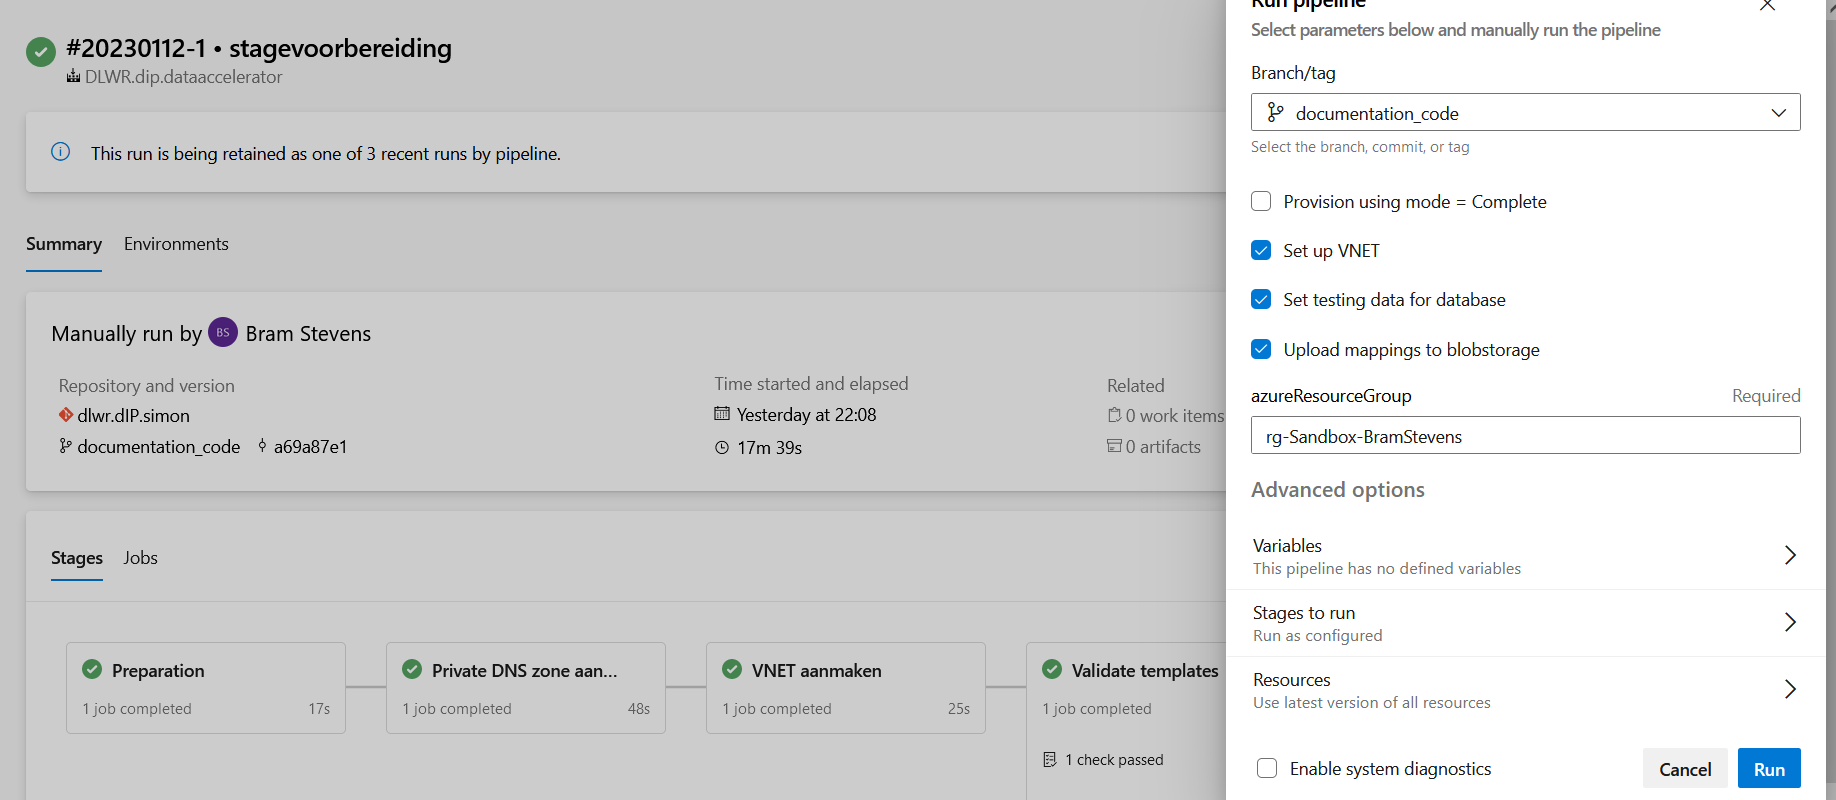
\includegraphics[scale=0.40]{../img/Pipeline.png}
    \caption{\label{fig:Opties}Azure pipeline opties}
\end{figure}

Deze wordt opgevolgd door een check  van de AIS deployment resources en worden deze ook aangemaakt. Hierbij wordt een Azure CLI script uitgevoerd die een Resource Group creëert binnen de gespecifieerde locatie.

Daarna wordt ook via de Azure CLI een Private DNS zone opgesteld binnenin de Resource Group volgens de naamgeving die in de parameters meegegeven is. Dit wordt opgevolgd door het aanmaken van een Virtual network via de Azure CLI die dan de correcte naamgeving voorziet evenals de Resource Group, locatie en subnetten die meegegeven worden bij de variabelen die naar wens kunnen aangepast worden.

De hier op volgende stage binnen de pipeline spitst zich toe op het valideren van de BICEP templates. Dit gebeurt op basis van enkele testen die uitgevoerd worden en de syntax die nagekeken wordt. Op deze manier kunnen fouten in de BICEP bestanden vroeg in het proces gedetecteerd en aangepakt worden.

De provision stage maakt dan alle resources aan binnen de omgeving volgens de BICEP templates die opgesteld zijn. Dit proces neemt het grootste deel van de uitvoering in beslag maar verloopt ook volledig automatisch.

Het deel dat hierop volgt slaat het PowerShell bestand dat benodigt is al men de databank wilt vullen op in het Storage Account en voert deze dan ook uit indien de optie geslecteerd is. Deze is zichtbaar in bijlage B.9 PowerShell. Dit script is ook personaliseerbaar via de variabelen die gebruikt worden in de pipeline en zijn doorgegeven aan het script om de correcte connectionstring op te stellen om toegang te verkrijgen tot de databank. Er werd in dit geval gekozen voor PowerShell omdat via YAML zelf of de Azure CLI het niet mogelijk was de databank te voorzien van correcte data. Deze werdt via een URL opgehaald en in de databank toegevoegd op basis van de parameters.

Ten laatste worden de overige bestanden, namelijk die XSLT mappings en queries ook indien de optie geslecteerd is, in het Storage Account opgeslagen zodat men kan gebruik maken van XSLT met de Data-Accelerator.

Deze stappen worden dan bij de opstart van de pipeline doorlopen op basis van geselecteerde opties zoals verduidelijkt bij de pipeline. Dit proces neemt gemiddeld een vijftiental minuten in beslag waarna de volledige omgeving aangemaakt is en bijna klaar is voor gebruik.
Het engiste dat nog moet gebeuren is de connectionstring naar de SQL databank en de Storage Account toevoegen bij de local settings van de Data-Accelerator. Als men nu de accelerator laat draaien kan men via gepersonaliseerde requests data opvragen en bewerken uit de gecreëerde databank. Van hier uit wordt er bekeken hoe men extra functionaliteit omtrent GraphQL of gelijkmatige Azure toepassingen kan toevoegen. Op die manier wordt de volgende deelvraag beantwoord: "Welke integratie mogelijkheden zijn er voor GraphQL binnen een Data-Accelerator omgeving?"

\subsection{\IfLanguageName{dutch}{Implementatie GraphQL}{Implementatie GraphQL}}%
\label{sec:Implementatie GraphQL}

Om GrapQL toe te voegen aan de werkomgeving gaat men naar de aangemaakte Resource Group en kan men de API Management module toevoegen.
Hierbij selecteerd men de Resource Group en de naam die de werkomgeving moet krijgen. Dit is te zien in Figuur~\ref{fig:APIM}.
Bij de optie Monitoring kan men de Application insight selecteren die via de pipeline opgezet is, op deze manier wordt er ook monitoring toegevoegd aan de module. Bij de optie Virtual network kan met de opgezette virtuele netwerken en endpoints toevoegen indien dit gewenst is. Binnen deze bachelorproef is dit geen vereiste. Als dit naar wens ingevuld is creëerd men de module. Het resultaat is te zien in Figuur~\ref{fig:APIS}.

\begin{figure}
    \centering
    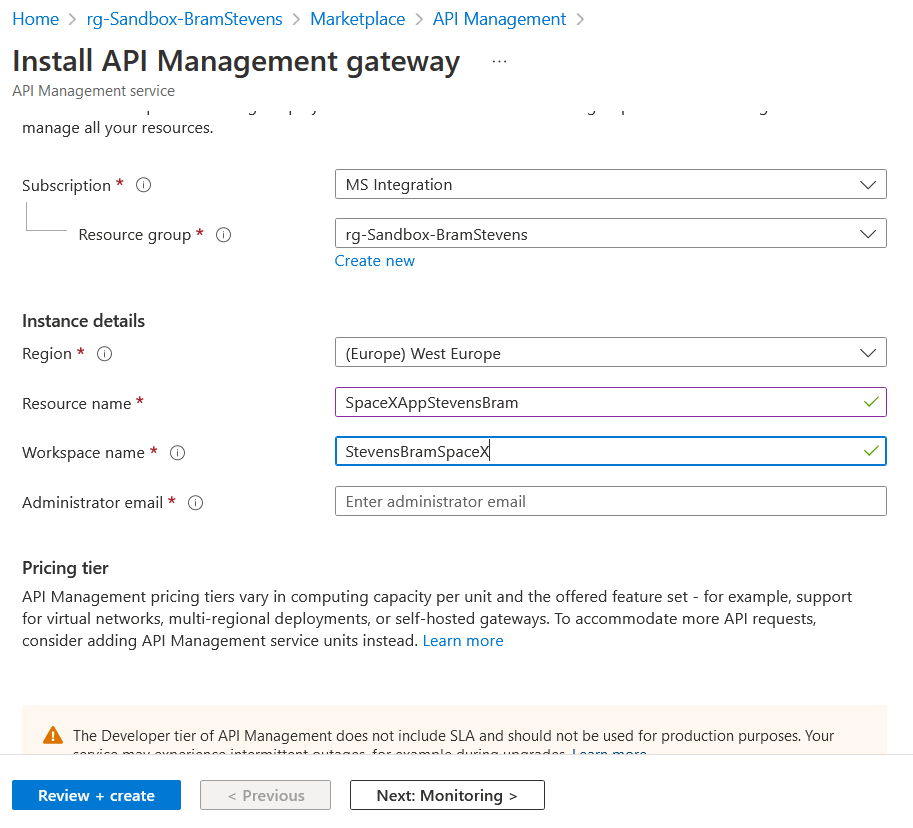
\includegraphics[scale=0.60]{../img/APIManagement.png}
    \caption{\label{fig:APIM}API Management config}
\end{figure}

\begin{figure}
    \centering
    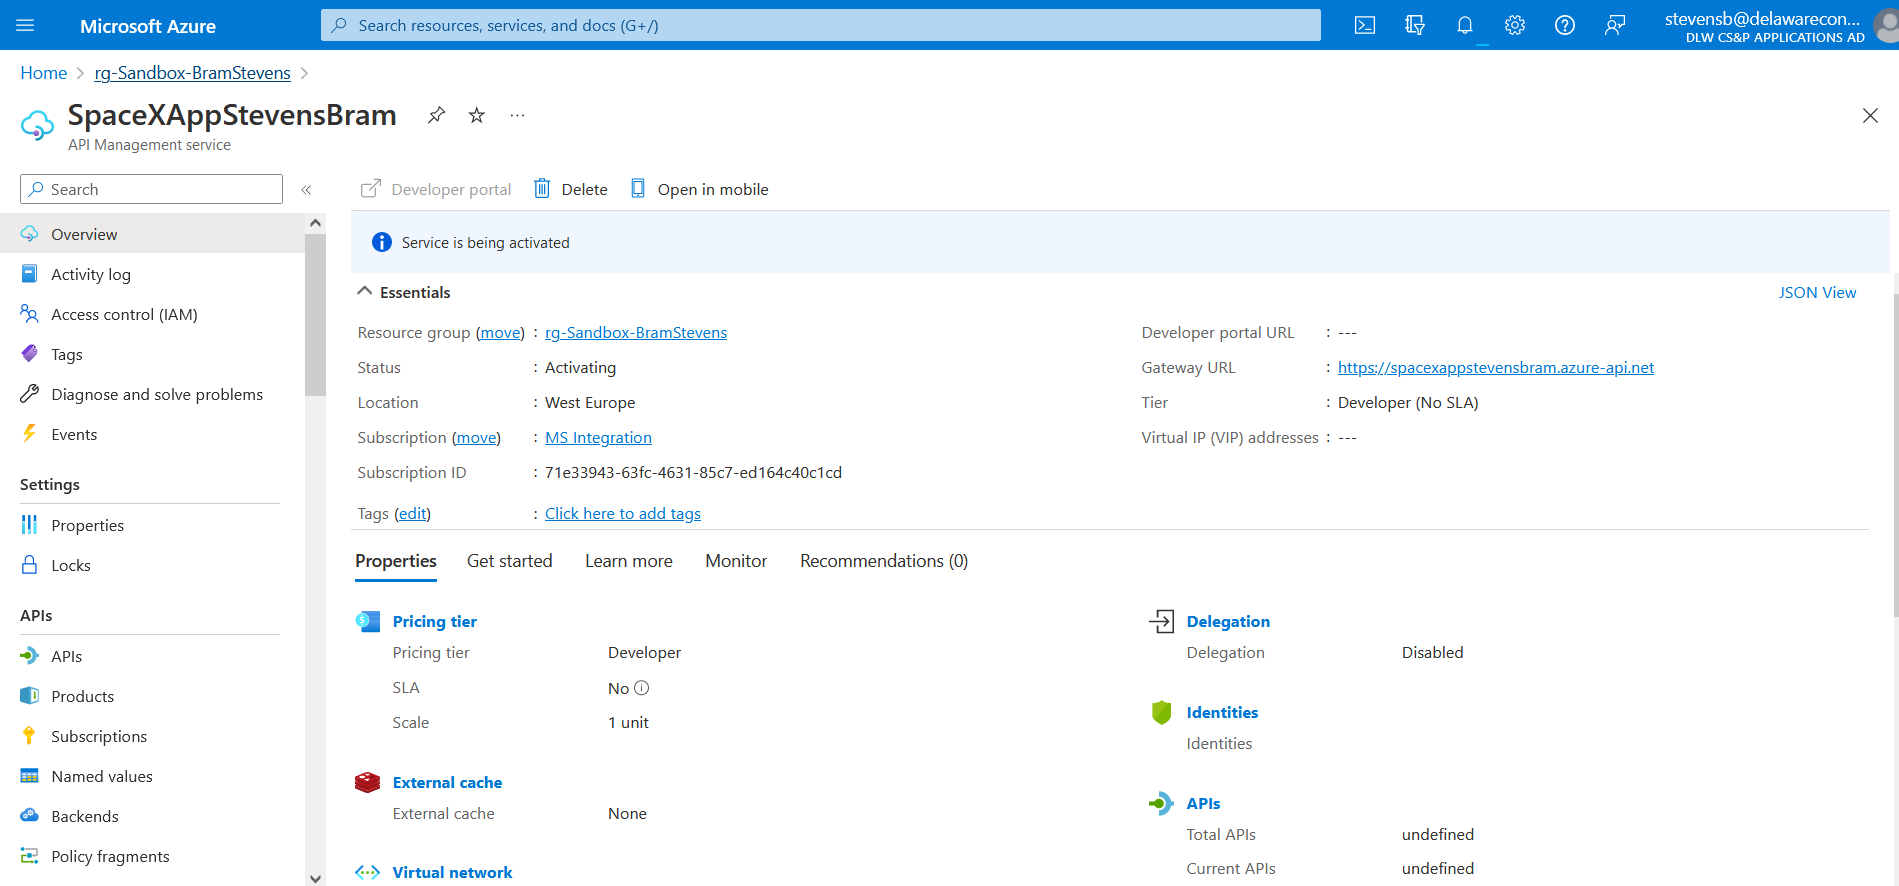
\includegraphics[scale=0.40]{../img/APIService.png}
    \caption{\label{fig:APIS}API Service overview}
\end{figure}

Vervolgens importeert men de benodigde API via de optie in de linker kolom genaamd APIs. In dit menu kan men ook kiezen voor de optie om een nieuwe API aan te maken via de optie Define a new API en de optie GraphQL te selecteren of om een synthetische GraphQL API te creëren en een bijhorend schema bij te voegen. Dit kan ook een gekozen endpoint zijn, Logic of Function App.

Na het creëren van de API kan deze geselecteerd worden en ziet men het scherm dat te vinden is in Figuur~\ref{fig:API}. Hier kan men policies toevoegen en de API testen. Dit gebeurd via de Add inbound policy en te selecteren welke toepassing er benodigt is. Dit bevat onder andere het filtreren van IP adressen en limitaties toevoegen ten opzichte van het aantal requests die tot de backend geraken. Deze kunnen ook verder gepersonaliseerd worden door XML code.

\begin{figure}
    \centering
    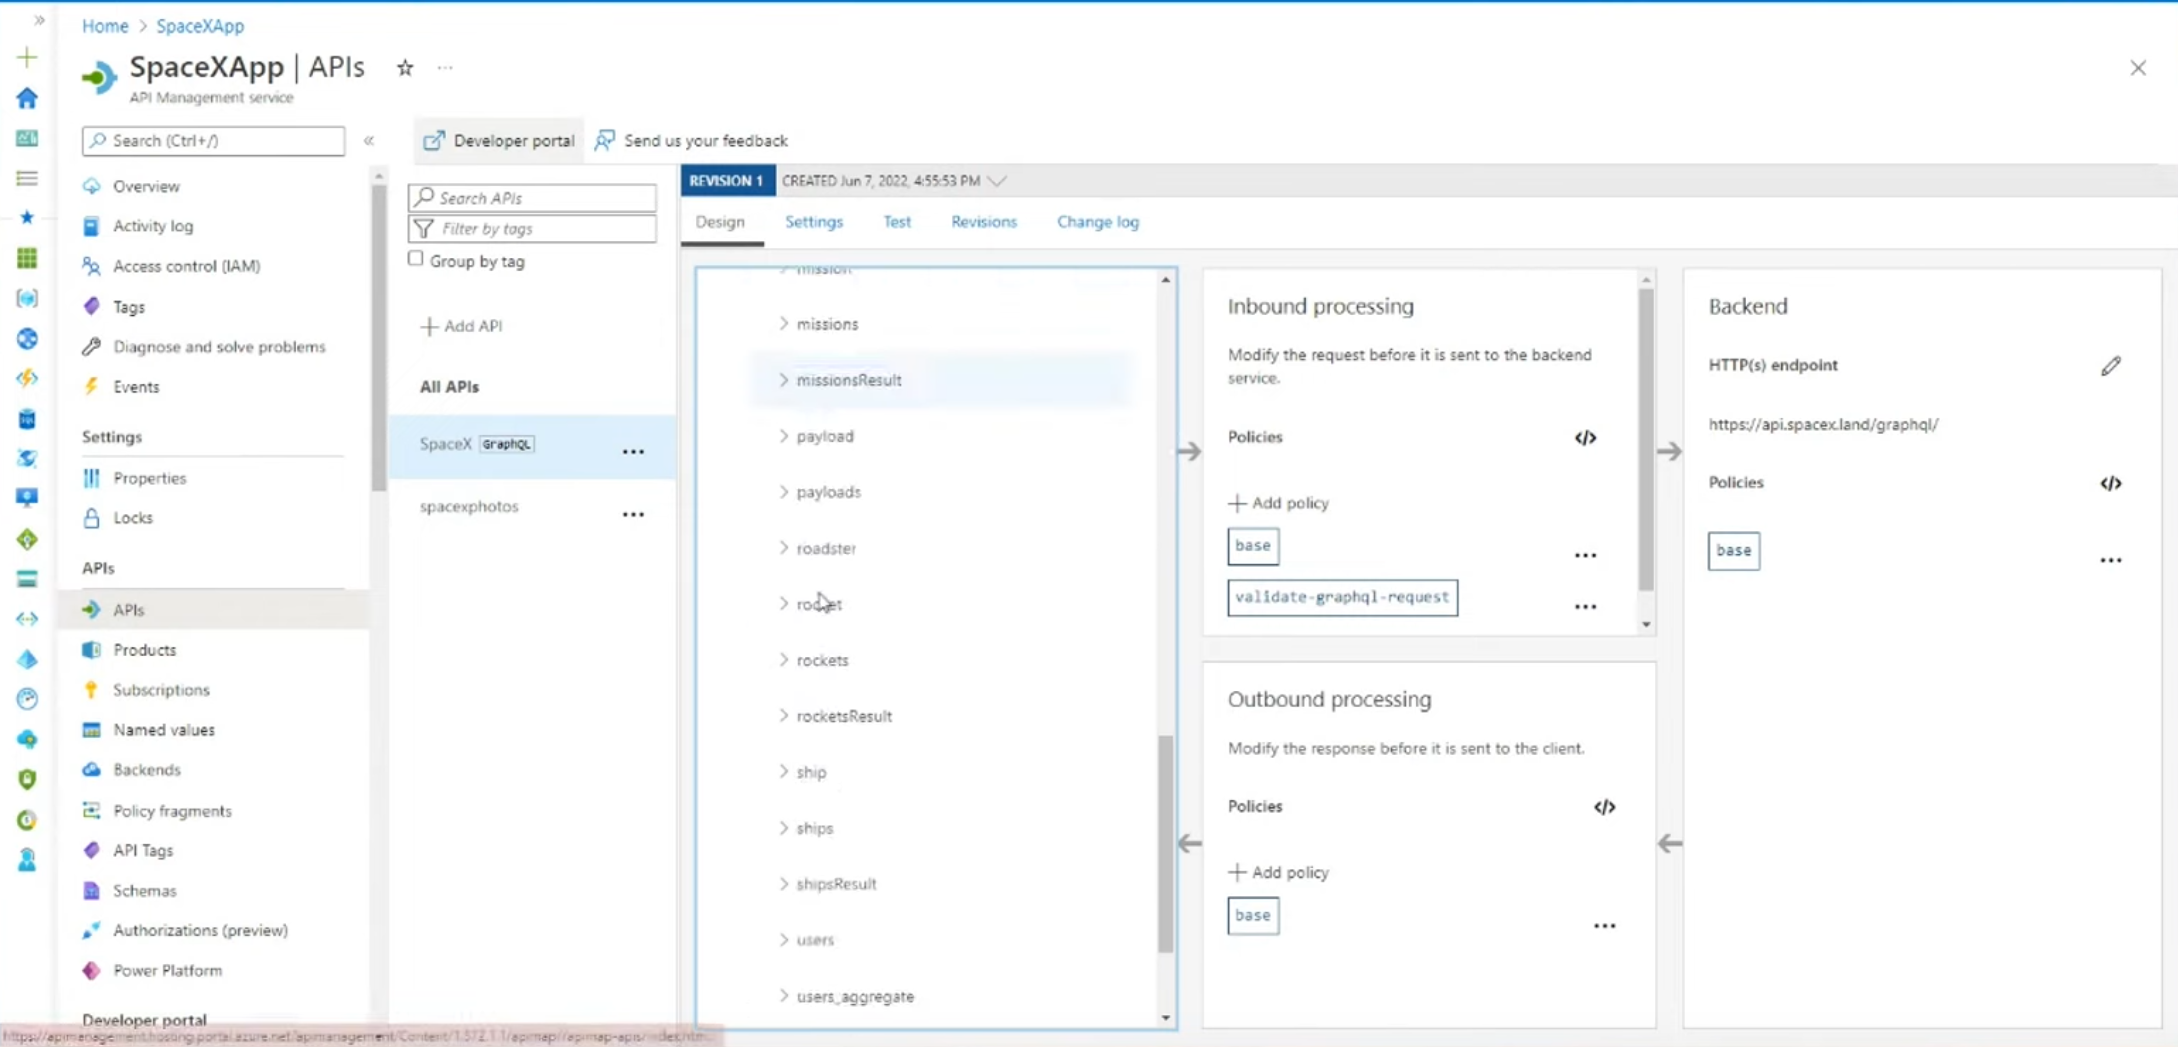
\includegraphics[scale=0.40]{../img/API.png}
    \caption{\label{fig:API}API overview}
\end{figure}

Op voorgaand uitgelegde manier kan men dus eenvoudig GraphQL functionaliteit toevoegen aan een opgestelde omgeving binnen Azure en meteen gebruiken in samenhang met een Data-Accelerator omgeving. Zo is ook de laatste deelvraag beantwoordt: "Kan een Data-Accelerator GraphQL benutten?" Eenmaal de omgeving opgesteld is via de pipeline kan men op slechts enkele minuten tijd GraphQL ondersteuning toevoegen aan de gewenste data zijnde Logic en Function Apps of een endpoint van een bestaande API.

%% TODO: Hoe ben je te werk gegaan? Verdeel je onderzoek in grote fasen, en
%% licht in elke fase toe welke stappen je gevolgd hebt. Verantwoord waarom je
%% op deze manier te werk gegaan bent. Je moet kunnen aantonen dat je de best
%% mogelijke manier toegepast hebt om een antwoord te vinden op de
%% onderzoeksvraag.



